The project aims to solve an OpenAI gym environment from the control section that can be seen here \href{https://gym.openai.com/envs/#classic_control}{Control Environments}. The environment selected is the MountainCar-v0 because it has a continuous state space with a deterministic action space being a good candidate for applying deep q learning. The details of the problem are as follows:
\begin{itemize}
\item \textbf{Task:} MountainCar-v0
\item \textbf{Category:} Classic Control
\item \textbf{Goal:} Get an under powered car to the top of a hill (top = 0.5 position) by creating momentum as shown in Fig.\ref{fig:car}
\begin{figure}[h]
\centering
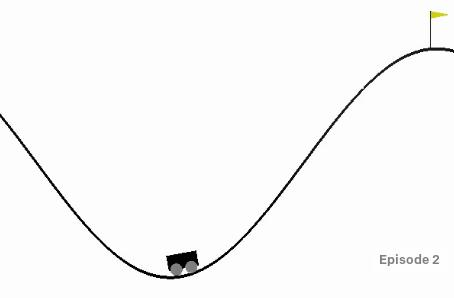
\includegraphics[width=0.8\textwidth]{environment.jpg}
\caption{\label{fig:car} Mountain Car environment}
\end{figure}
\item \textbf{State Space:}
      \begin{table}[h]
      \centering
      \begin{tabular}{|c|c|c|c|}
      \hline
      \textbf{Num} & \textbf{Observation} & \textbf{Min} & \textbf{Max} \\ \hline
      0            & position             & -1.2         & 0.6          \\ \hline
      1            & velocity             & -0.07        & 0.07         \\ \hline
      \end{tabular}
      \caption{State Space}
      \label{tab:1}
      \end{table}
\item \textbf{Action Space:}
		\begin{table}[h]
        \centering
        \begin{tabular}{|c|c|}
        \hline
        \textbf{Num} & \textbf{Observation} \\ \hline
        0            & push left            \\ \hline
        1            & no push              \\ \hline
        2            & push right           \\ \hline
        \end{tabular}
        \caption{Action Space}
        \label{my-label}
        \end{table}
\item \textbf{Termination Criteria:} The episode ends when either the goal is reached or 200 actions are made.
\item \textbf{Rewards:} -1 penalty for each environment step until termination criteria is met.
\item \textbf{Potential Solution:} Since the environment has continuous state space and discrete action space a good candidate would be a \textbf{Deep Q Network}
\end{itemize}